% !TEX encoding = UTF-8 Unicode 

\title{Aktuelle Themen des Software-Engineerings\\Statische Analyse}
\author{
Dominik G\"atjens \\
Manuel Henle \\
\and
Patrick Nisch \\
Patrick Permien
}
\date{\today}
\documentclass[12pt,twocolumn]{article}
% encoding:
\usepackage[utf8]{inputenc}
\usepackage[T1]{fontenc}
\usepackage[german]{babel}
\usepackage[authoryear]{natbib}
\usepackage[hyphens]{url}
\usepackage{hyperref}
\usepackage{graphicx}
\usepackage{enumitem}
\usepackage{listings} \lstloadlanguages{}


\begin{document}
\setlist{noitemsep} % no space between items in enumerate/itemize
\onecolumn
\maketitle

\begin{abstract}

Die statische Code-Analyse ist ein Verfahren zur formalen Prüfung des Quellcodes.\\Zu dieser Art der Code-Analyse gehören Methoden und Techniken, die gewährleisten, dass die entwickelte Software den geforderten Qualitätsanforderungen erfüllt. Die Bandbreite reicht von einfachen Überprüfungen des Code-Stils bis zu komplexen Untersuchung nach Speicherlecks. Nach einer Einführung in die Thematik folgt eine Beschreibung der Funktionsweise unterschiedlicher Methoden der Statischen Code-Analyse. In einer Übersicht werden verschiedene und in der Praxis häufig eingesetzte Tools dargestellt. Eine abschließende Bewertung fasst den Mehrwert statischer Code-Analysen zusammen und hilft den Nutzen des Verfahren richtig beurteilen zu können.
\end{abstract}
\twocolumn
\section{Einleitung / \"Uberblick}
Die statische Analyse, auch Quellcode Analyse, ist ein statisches Software-Testverfahren. Sie ist ein erster und unverzichtbarer Schritt verschiedenster Software-Qualitäts-Kontrollen. Dabei wird ein Verständnis für die Code-Struktur hergestellt. Sie trägt dazu bei, den Code an definierte Standards anzupassen.

Die Analyse ermöglicht eine frühzeitige Erkennung und somit die Korrektur von Fehlern mit geringerem Aufwand. Durch das frühe Eingreifen wird verhindert, dass scheinbar kleine Fehler sich manifestieren und Wochen, Monate oder Jahre später zu erheblichen Problemen führen.

Bei der statischen Analyse wird -- im Vergleich zu dynamischen Testverfahren -- die zu testende Software nicht ausgeführt. Da der Quelltext benötigt wird, lässt sich die statische Analyse den White-Box-Testverfahren zuordnen.

Die Analyse kann vollständig manuell durchgeführt werden; dies ist aber mit erheblichem Aufwand verbunden. Daher werden automatisierte Tools eingesetzt. Das erste Tool dieser Art war ``Lint'', das in den 1970er Jahren von den Bell Labs für die Programmiersprache C entwickelt wurde. Das heutzutage bekannteste Tool ist ``FindBugs'', auf dessen Funktionsweise und Umfang wir später noch näher eingehen. Im Vergleich zu den frühen automatisierten Hilfen wird heute neben funktionalen Fehlern auch sogenannter ``Code-Smell'' erkannt. Dies können beispielsweise duplizierter oder ``toter Code'' (nicht-verwendeter Code) sein. Dabei kommen Techniken wie die \emph{Taint-Analyse} oder die \emph{Datenflussanalyse} zum Einsatz.

Das Ziel der statischen Analyse ist momentan nur das Aufzeigen von möglichen Fehlern, es wird keine automatische Korrektur des Codes vorgenommen. Idealerweise würden solche Tools mit einem hohen Maß an Zuverlässigkeit mutmaßliche Fehler und Sicherheitslücken automatisch erkennen und beheben. Dies ist jedoch noch nicht realisierbar. Momentan gibt es noch immer eine hohe Rate von Fehleinschätzungen.

Nichtsdestotrotz ist die statische Analyse in der heutigen Programmierung nicht mehr wegzudenken und dient als hervorragende Hilfestellung für Programmierer und Tester um vor allem sicherheitsrelevante Teile des Codes zu analysieren und Fehler effizient zu finden.
Die Tools selbst lassen sich in der Regel problemlos in gängige Entwicklungsumgebungen integrieren und können somit unmittelbar während der Entwicklung den Programmierer auf eventuelle Fehler hinweisen.

\paragraph{Beispiele für erkennbare Fehler:}\footnote{vgl. \url{http://www.klocwork.com}, \url{http://www.hitex.com}}
\begin{itemize}
\item Syntaktische Fehler (z.B. Tippfehler, falsche Vergleiche, Klammersetzung)
\item Stilfehler, Einhaltung von Coding-Standards (z.B. Whitespacing)
\item Software Metriken
\item ``Bad Smells''
\item Leere Anweisungen (z.B. Exceptions)
\item Speicherlecks
\item Zerstörung von Speicherinhalten
\item Zugriffe über NULL-Zeiger
\item Index außerhalb der Grenzen
\item Unsichere Zeigerarithmetik
\item Benutzung von Speicher nach Freigabe
\item Inkonsistente Freigabe
\item Konstruktor-/Dekonstruktor-Lecks
\item Fehlerhafte Verwendung von virtuellen Member-Funktionen
\item Arithmetische Fehler
\item Nicht initialisierte / unbenutzte Variable
\item Redundanter / überflüssiger Code
\item Division durch null
\item 32/64-bit Kompatibilitätsprobleme
\item Pufferüberläufe
\item Nicht-validierte Benutzereingaben
\item Mögliche Sicherheitsproblematiken (z.B. Injections, Cross-Site-Scripting)
\item Veraltete Methoden
\item Gelockte und nicht-gelockte Zugriffe auf dieselbe Variable per Threads
\item Endlosschleifen
\item Toter Code
\item Unerreichbarer Code
\end{itemize}

\paragraph{Stärken, Schwächen und Grenzen der statischen Analyse:}\footnote{vgl. \url{https://www.owasp.org/index.php?title=Static_Code_Analysis\&oldid=132351}}
\subparagraph{Stärken:}
\begin{itemize}
\item Skaliert sehr gut
\item Sehr Hilfreich sowohl bei einfachen Fehlern (z.B. Tippfehler) als auch bei komplexeren Interaktionen (z.B. Pufferüberläufe, SQL-Injections, etc.)
\end{itemize}

\subparagraph{Schwächen:}
\begin{itemize}
\item Viele Sicherheitslücken sind sehr schwer automatisch zu finden, z.B. bei Authentifizierung, Zugriffskontrollen, unsichere Verwendung von Kryptographie, etc.
\item Hohe Falsch-Positiv-Rate
\item Konfigurationsprobleme können nicht bzw. nur schwer erkannt werden
\item Schwer nachzuweisen, dass ein gefundenes Sicherheitsproblem eine tatsächliche Gefährdung darstellt
\item Schwierigkeiten bei der Analyse von Codestücken, die nicht kompiliert werden können, z.B. wenn entsprechende Referenz-Bibliotheken nicht mitgeliefert wurden zum Testen
\end{itemize}

\subparagraph{Falsch Positiv:}
Eine statische Code Analyse führt häufig zu falsch eingeschätzten positiven Ergebnissen, bei denen das Tool eine Schwachstelle aufzeigt, welche eigentlich keine ist. Das tritt auf, wenn das Tool die Integrität und Sicherheit des Datenflusses durch die Applikation von Eingang zum Ausgang nicht immer nachvollziehen kann. Beispiele dafür sind, wenn Programmcode analysiert wird, welcher mit Closed-Source-Software oder externen Komponenten interagiert.

\subparagraph{Falsch Negativ:}
Falsch negativ Ergebnisse können ebenso auftreten, wenn Schwachstellen auftreten, diese aber nicht vom Tool gemeldet werden. Dies kann dann vorkommen, wenn eine neue Schwachstelle in einer externen Komponente entdeckt wurde oder das Tool keine Kenntnis von der Laufzeitumgebung hat und ob diese sicher konfiguriert wurde.

\paragraph{Abgrenzung zu Code Reviews:}
Statische Analyse darf nicht verwechselt werden mit Code Reviews. Die Analyse kann Teil eines Review Prozesses sein und optimiert diesen insofern, dass durch die vorgeschlagenen Verbesserungen der Code syntaktisch korrekt und übersichtlich vorbereitet ist.

Ein Code Review geht prinzipiell noch einen Schritt weiter und verfolgt teilweise auch andereweitige Ziele. So prüft eine statische Analyse beispielsweise, ob eine Funktion generell dokumentiert ist, bei einem Code Review wird zusätzlich betrachtet, ob die Funktion ausreichend und verständlich erklärt wurde.

Somit ist ein Code Review immer eine manuelle Prüfung des Quellcodes durch mindestens eine weitere Person. Dabei wird die Aufmerksamkeit auf Punkte wie die Verständlichkeit des Codes oder sinnvoll benannte Variablen gelegt. Ebenso können Verbesserungen im Code bzw. in dessen Struktur und mögliche alternative Lösungsansätze betrachtet werden.


% !TEX encoding = UTF-8 Unicode 
\section{Werkzeuge}

\paragraph{Grundlegende Ansätze:} An erster Stelle steht in der Programmierung hinsichtlich der statischen Code-Analyse zunächst das kritische Hinterfragen der Qualität des eigenen Quellcode bezüglich der technischen Korrektheit und der  Erfüllung der eigenen oder firmenweiten Vorgaben für guten Programmierstil. Diese Überprüfung ist gerade für erfahrene Programmierer Routine. Umfangreiche Nachschlagewerke geben Ratschläge zur Optimierung von Quellcode, zum Beispiel \cite{mcconnell2004}.

Die Überprüfung muss nicht immer durch den Programmierer selbst erfolgen, sondern kann auch in Form von Code Reviews mit unterschiedlichem Grad an Formalisierung organisiert sein \citep{spillner2011}. Reviews können über das Web auch zeitlich und örtlich verteilt stattfinden \citep{codereviews:meyer}.

Komplexere Entwicklungsumgebungen liefern teilweise Analysetools standardmäßig mit. Eclipse ist ein gutes Beispiel hierfür.

Eine weitere, ebenfalls noch sehr einfache Stufe der statischen Code-Analyse, stellt bei kompilierten Sprachen zunächst der Compiler dar. Dieser gibt auch ohne den Einsatz von zusätzlichen Analysewerkzeugen Hinweise auf schlechten Programmierstil oder mögliche Laufzeitprobleme. Beispielsweise weist der Java-Compiler den Programmierer auf nicht erreichbaren Code hin -- also Code der in einem Block mit nicht erfüllbarer Vorbedingung steht.

\paragraph{Bekannte Tools:} Als Werkzeuge zur statischen Code-Analyse sind in der Vorlesung in erster Linie \textit{FindBugs} und \textit{CheckStyle} besprochen worden, die beide im Java-Bereich eingesetzt werden. Für Java ist zudem \textit{PMD} erwähnenswert; das derzeit wohl neueste Werkzeug ist ``\textit{Development Testing}'' von coverity \citep{neumann2012}\footnote{\url{http://www.coverity.com/development-testing/index.html}}. Es existiert eine Vielzahl weiterer Tools\footnote{\url{http://en.wikipedia.org/w/index.php?title=List_of_tools_for_static_code_analysis\&oldid=500773445}}, die für andere Sprachen, Entwicklungsumgebungen oder nur bestimmte Plattformen entwickelt sind. Dazu zählen \textit{StyleCop}, Microsoft \textit{fxCop} und Jetbrains \textit{ReSharper} für alle bzw. einige der .NET-Sprachen. Eines der ersten Werkzeuge für die statische Analyse war \textit{Lint} bzw. \textit{Splint} für die Sprache C. Hinzu kommt Software, die  Code Coverage Analysen im Zusammenspiel mit Komponententest-Frameworks erstellt; hierzu zählen u.a. \textit{Emma} für Java und Jetbrains \textit{dotCover} für die .NET-Sprachen.


In Abbildung \ref{fig:eclipse-cs} auf Seite \pageref{fig:eclipse-cs} ist exemplarisch die Anwendung von Checkstyle mithilfe des eclipse-cs-Plugins\footnote{\url{http://eclipse-cs.sourceforge.net/}} für die Eclipse-IDE dargestellt. Abbildung \ref{fig:eclemma} (S. \pageref{fig:eclemma}) zeigt die Eclipse-Integration von Emma durch das Plugin Eclemma\footnote{\url{http://eclemma.org/}} im Zuge einer Code Coverage-Analyse.


\paragraph{Leistungsspektrum:} Teilweise decken die Werkzeuge in ihrem Leistungsspektrum ähnliche oder gleiche Anforderungen ab wie ihre Konkurrenten. Die Mehrzahl der genannten Werkzeuge fügen sich in die Entwicklungsumgebung als Plugin ein und können in den Analysen durch Konfigurationen individualisiert werden. 

Die Aufgaben von Software für die statische Analyse umfassen hauptsächlich:
\begin{enumerate}
\item das Aufdecken von Fehlern und typischen Fehlermustern bzw. -quellen,
\item die Analyse von Anweisungen und Aufrufen von Methoden,
\item die Analyse des Datenflusses und
\item die Prüfung, ob heikler oder sicherheitskritischer Code vorhanden ist. 
\item Die Prüfung auf Auffälligkeiten, wie \begin{enumerate}
\item stilistische Unzulänglichkeiten oder
\item Möglichkeiten zur Performance-Optimierung,
\end{enumerate} können je nach Leistungsumfang des Tools hinzukommen.
\end{enumerate}

Eine Beschreibung der Ziele statischer Analyseverfahren findet sich sowohl in eher theoretisch \citep[S. 270]{liggesmeyer2009} als auch in praktisch orientierter Fachliteratur \citep[S. 98]{linz2010}. Die Aufgaben der Werkzeuge leiten sich daraus unmittelbar ab.

Die Konfiguration der Werkzeuge lässt üblicherweise das Festlegen genereller, projektspezifischer und individueller Regeln zu, um die Priorität von Warnungen anpassbar zu machen, und um Warnungen ganz zu vermeiden die den Programmierer nicht interessieren.

Je nach Tool ist es möglich, die toolgestützten Inspektionen der statischen Analyse im Rahmen eines Build-Prozesses mit z.B. Ant oder Maven\footnote{} einzubinden. Auch Kopplungen mit Continuous Integration Services sind, z.B. als Plugin, auf dem Markt erhältlich.

\paragraph{VCS:} Je nach Projektvorgaben ist es bei einigen der Softwaretools möglich, das Bereitstellen von Quellcode in die gemeinsam genutzte Versionsverwaltung zu verweigern, wenn der Code nicht den im Vorfeld definierten Mindestanforderungen genügt, die im Zuge der statischen Analyse vom Werkzeug geprüft werden. Die Vorlesung hat aufgezeigt, dass dieser Ansatz in der Praxis kritisch hinterfragt werden muss, um nicht das Gefühl von Überwachung oder Gängelung aufkommen zu lassen.


\section{Funktionsweise der Werkzeuge}

Dieses Kapitel wird sich mit der internen Funktionsweise der gebräuchlichsten statischen Code Analyse Tools für Java beschäftigen. Diese sind wie in vorherigen Kapiteln dargestellt: Findbugs, Checkstyle, PMD sowie Emma, welches den Code zwar nicht statisch analysiert, im Rahmen der Vorlesung aber trotzdem im Context der statischen Analyse besprochen wurde.


\subsection{FindBugs}

FindBugs ist ein von der Universität von Maryland initiiertes Software-Projekt zur statischen Code Analyse. FindBugs genießt große Verbreitung in der Industrie und wird von Firmen wie Google und ehemals Sun Microsystems nun Oracle unterstüzt.
FindBugs arbeitet vollständig auf dem Java-Bytecode und kann dadurch auch auf "binären" Projektdistributionen durchgeführt werden. 

FindBugs bietet eine große Anzahl an mitgelieferten Fehler-Pattern, die in verschiedene Warnstufen eingeteilt sind. Ihr Hauptfokus liegt auf der Erkennung von fehlerhaftem Code, der bei der Ausführung zu Runtime-Fehlern führen würde.

Möchte man seine eigenen Fehler-Pattern hinzufügen, bietet Findbugs dafür ein Plugin Konzept, welches allerdings ein Verständnis der internen Funktionsweise von FindBugs voraussetzt.
 
FindBugs nutzt für die ByteCode Analyse die Apache BCEL Library, welche eine gut nutzbare Schnitstelle zu komplierten Java Class Files bietet, welche in vielen Bytecode-nahen Projekten eingesetzt wird.

Dies kann für Entwickler einen großen Nachteil bedeuten, da die wenigstens ein Verständnis von ByteCode haben. Man muss beachten, dass die baumartige Struktur des Sourcecodes im Bytecode, wie auch in Maschinensprache, zu einer flachen sequenziellen Abfolge von Instruktionen wird. 

Weiter erschwert das Erstellen eines eigenen Fehler-Pattern, dass der Bytecode sequenziell Durchlaufen wird und der Bytecode Scanner dabei bei jeder Instruktion die ihm zugeordnenten Fehler-Detectoren über ein Visitor-Pattern aufruft. 
Dadurch ist der Entwickler des Fehler-Detektor dafür verantwortlich, sich die bereits gescannten Instruktionen in seinem State zu speichern. Hierfür bietet sich i.d.R. eine Statemaschine an. Aber auch dies ist ein Programmierparadigma, das bei vielen Entwicklern in Zeiten von OOP nicht mehr häufig genutzt wird und somit eine weitere Hürde in der Erstellung von eingenen Fehler-Mustern darstellt.

Die Analyse des Bytecodes hat aber auch positive Seiten. So ist zum einen die Analyse sehr perfomant, da sie einfach einer linearen Abarbeitung von Instruktionen entspricht und zum anderen ist die der Bytecode bereits durch den Java Compiler optimiert worden und somit verringert sich die Häufigkeit eines False-Positives.

In der Usability bietet FindBugs auch Vorteile gegenüber anderen Tools. So bietet es zum einen eine sehr gute und aktuelle Integration in viele Eclipse und viele andere Entwicklungsumgebungen und lässt sich zum anderen über ein Konsolen-Tool einfach in automatische Build-Prozesse einbinden.


\subsection{PMD}
PMD, dessen Name nach eigenen Aussagen des Projekts keine ausgeschriebe Bedeutung hat, ist ebenfalls ein Werkzeug zur statischen Code Analyse von Java-Code. 

PMD liefert ebenfalls eine Vielzahl an eingebauten Regeln, die anders als bei FindBugs nicht so sehr auf potentielle Fehler, sondern eher auf ineffizenten Code ausgelegt sind. Beispiele hierfür sind z.B. leere Blöcke, toter Code oder die falsche Verwendung von Strings und StringBuffern. 

PMD besitzt weiter einen Copy/Paste Detector, der es erlaubt, mit des Rabin-Karp-Algorithmuses duplizierten Code zu finden.

PMD operiert, anders als FindBugs, nicht auf den binären Java Class Files, sondern auf dem Source-Code. Genauer gesagt, auf dem Abstract Syntax Tree, der aus dem Source-Code vor dem Erstellen des Bytecodes erzeugt wird. 

Die Analyse des ASTs ist zwar nich so performant, wie das einfache Scannen von Bytecode, besitzt für das Entwicklen von eigenen Regeln aufgrund der Nähe zum Sourcecode aber entsprechende Vorteile.

Bei der Transformation von Quelltext zu einem Abstract Syntax Tree gehen (im Gegensatz zu Bytecode) keine Informationen über die Struktur des Quelltextes verloren. Es wird einzig der vorhandene Quelltext in einem Baum abgebildet. 
Möchte man nun seine eigenen PMD Regeln hinzufügen, reicht es aus den AST zu travasieren und auf das Vorkommen des entsprechenden Musters zu untersuchen. PMD bietet für diese Aufgabe ein eigenes Entwicklungstool an, dass den erzeugten AST darstellt, und in dem man explorativ dieses Baum travasieren kann.

\begin{figure}[htbp]
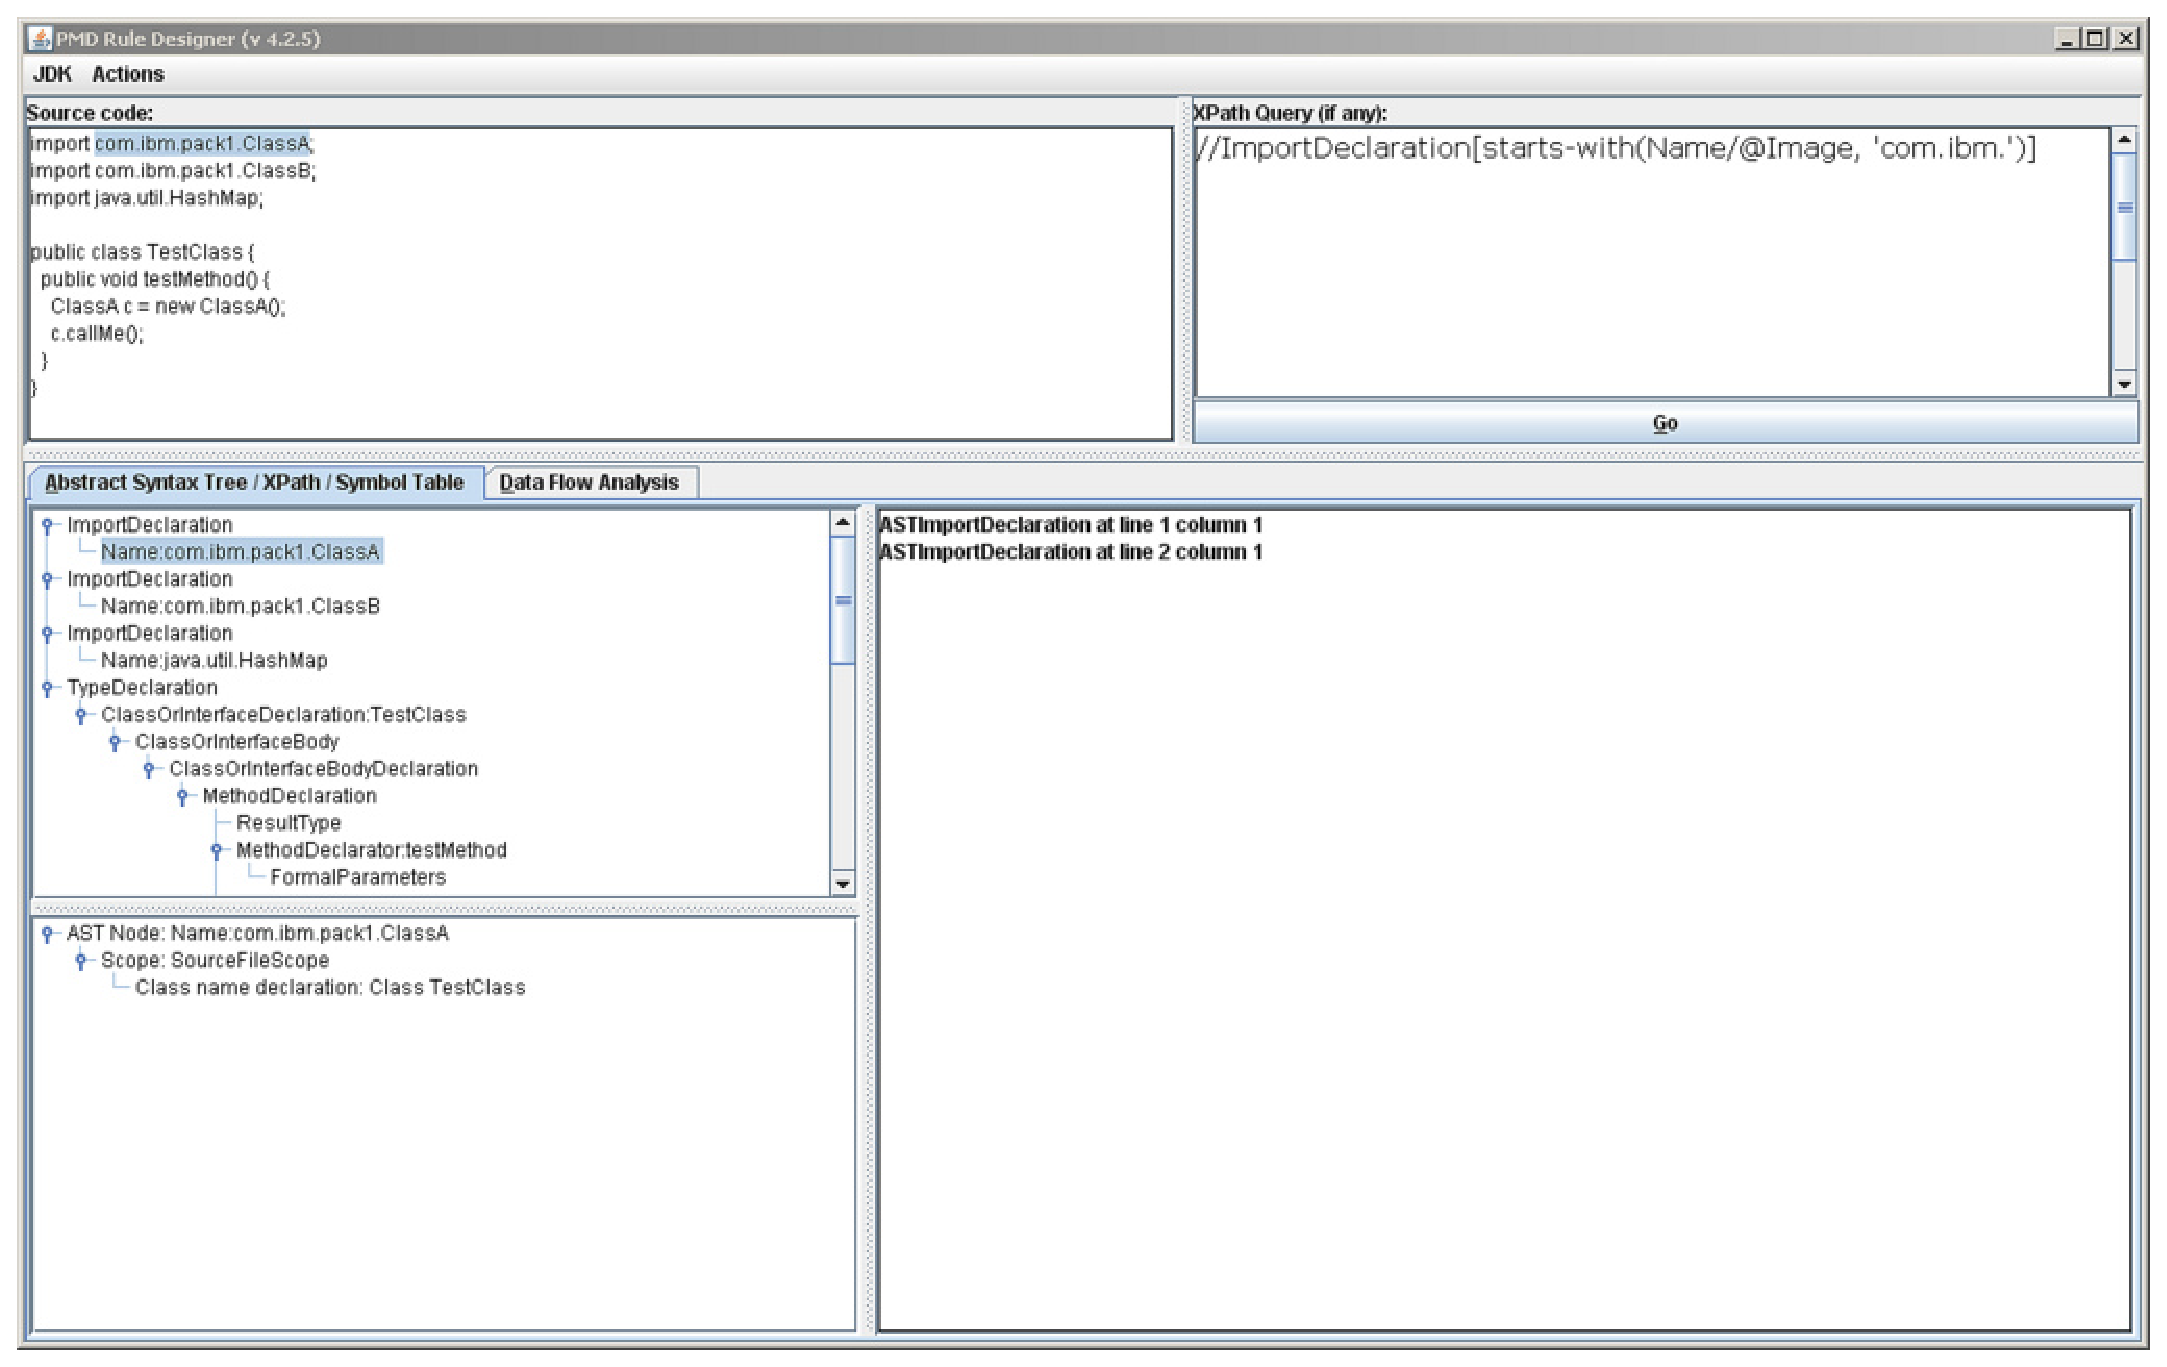
\includegraphics[width=10cm]{pmd-dev}
\caption{PMD Entwicklungs Werkzeug}
\end{figure}

Die Analyse auf einem AST bietet einen weiteren Vorteil. Da Bäume eine weit verbreitete Darstellungsform sind, gibt es bereits eine vielzahl von Werkzeugen die auf Ihnen operrieren können. Das in diesem Kontext wichtigste ist XPath.

PMD bietet neben der Schnitstelle für in Java implementierte Regeln, ebenfalls eine Schnittstelle für XPath. 

XPath oder auch XML Path Language ist eine vom W3-Konsortium entwickelte Abfragesprache, um Teile eines XML-Dokumentes (welches ebenfalls Bäume sind) abzufragen. Dabei bietet es eine sehr einfache Möglichkeit, Bäume zu travasieren.

\begin{lstlisting}
//child:Buch[count(./Seite)<=100]
/count(.Seite)>=10]
\end{lstlisting}

Das Beispiel würde z.B. alle Bücher aus einem Baum liefern, das maximal 100 doch mindestens 10 Kindelemente/Seiten hat.

Diese XPath-Ausdrücke können direkt in den PMD-Konfigurations-Files angegeben werden und machen es so für einfache und mittel komplexe Regeln überflüssig, eigene Java-Module zu implementieren.

PMD besitzt ebenfalls ein Konsolen-Tool, das sich sehr gut in den Build-Prozess integrieren lässt. Das entsprechende Eclipse Plugin ist zum Zeitpunkt dieses Papers leider nicht auf dem aktuellsten Stand und nutzt noch PMD Version 4, welche zur Version 5 inkompatibele Konfigurations-Dateien besitzt. Soll also die aktuellste PMD Version 5 im Build-Prozess verwendet werden, müssen zwei Konfigurations-Dateien für Version 4 und 5 gepflegt werden.


\subsection{Checkstyle}

Checkstyle ist das dritte wichtige statische Code Analyse Tool in der Java-Welt. Der Fokus von Checkstyle liegt weder in der effizenten Nutzung der JVM noch in dem Auffinden von Programmierfehlern, sondern vor allem in der Prüfung eines einheitlichen Programmierstils. 
Dafür liefert Checkstyle viele Regeln von Haus aus mit, die in Form von Modulen gruppiert sind. Einige Beispiele an mitgliefierten Modulen sind:
\begin{itemize}
\item Class Design, welches Prüfungen zum Softwaredesign beinhaltet
\item Coding, welches allgemeine Codingguidelines pürft.
\item Javadoc Comments zum Prüfen der Vollständigkeit und der richtigen Formatierung von Javadoc-Kommentaren
\item Metrics zur Einhaltung diverser Sofwaremetriken
\item Naming Convetions, um die Einhaltung von Namenskonventionen zu prüfen
\item Whitspaces zur Prüfung des Quelltextes hinsichtlich Leerzeichen und korrekter Einrückung.
\end{itemize}
Checksyle arbeitet ähnlich wie PMD auf dem AST und kann durch eigene Java-Module, die ebenfalls auf dem AST arbeiten, erweitert werden. Checkstyle bietet zur Erweierung noch eine weitere sehr nützliche Schnitstelle. So bietet das Modul 'Regexp' es dem Entwickler an, eigene Regeln mithilfe von regulären Ausdrücken zu schreiben. Dies dürfte gerade beim Überprüfen von Codeguildelines oft als ausreichend empfunden werden und bietet eine sehr einfache Schnitstelle, um Checkstyle zu erweitern.

Checkstyle lässt sich wie PMD und FindBugs sehr einfach über ein Konsolen-Werkzeug in den Build-Prozess einbinden und bietet ein gut funktionierendes Eclipse-Plugin.


\subsection{Emma}

Emma ist eine Code Coverage Library von Vlad Roubtsov. Sie zählt eigentlich nicht zu den statischen Code Analyse Tools, soll aber, da sie im Rahmen der Vorlesung im Kontext solcher behandelt wurde, hier kurz erläutert und zur statischen Code Analyse abgegrenzt werden. 
Das Ziel von Emma ist zu analysieren, welcher Code durchlaufen wird. Diese Information ist zum Beispiel für die Ermittlung einer Testabdeckung sehr interessant. Emma untersützt dabei eine Vielzahl von Metriken, die aber in den entsprechenden Ausarbeitungen zum Thema Testabdeckung zu finden sind. In diesem Kontext soll nun auf die Funktionsweise von Emma eingegangen werden.

Wie bereits erwähnt, ist Emma kein Werkzeug der statischen Code-Analyse. Die Funktionsweise von Emma basiert auf der Instrumentierung von Java Bytecode. Dazu untersützt Emma zwei Verfahren. Zum einen kann in einem zweiten "compile" Schritt der Bytecode um entsprechende Hooks erweitert werden, die dem Emma Toolkit die nötigen Daten über den durchlaufenden Code geben, und zum Anderen kann die Applikation mit einem speziellen Emma-Classloader gestartet werden, der den geladenen Bytecode on-the-fly instrumentiert. Als nächstes wird ein Driver benötigt, der den Instrumentierten Code durchläuft. Dies kann sowohl durc ein manuelles bedienen der Applikation geschehen, als auch durch automatische Tests. Der am weitestverbreiteste Anwendungsfall ist wohl die bereits erwähnte Testabdeckung bei Unit-Tests. Aber als reines Code Coverage Tool ist Emma natürlich wesentlich vielseitiger. So kann ein weiterer Interessanter Ansatz sein, dass man sich in (geerbtem) Spagetthi-Code einen schnellen Überblick verschaffen will, welcher Code bei einer Benutzeraktion durchlaufen wird.

Emma lässt sich über Ant und Maven Plugins gut in den BuildProzess inegrieren und bietet gerade für den Fall der Testabdeckung mit EclEmma ein sehr gutes Eclipse Plugin.



\section{Bewertung}
Viele Tools lassen sich einfach in gängige Entwicklungsumgebungen einbinden und brauchen nur wenig Einarbeitungszeit. Gleichzeitig liefern sie einen hohen Nutzen für die Entwickler. Der Quellcode kann direkt analysiert werden und der Entwickler erhält eine direkte Rückmeldung. Die Automatisierung des Tools führt zu sauberem Code und verbessert dadurch die Wartbarkeit.

Des Weiteren ist es empfehlenswert, sich mit den Tools zur Erhöhung der Sicherheit des Codes zu befassen und diese als Teil des Entwicklungsprozesses einzubinden. Den größten Nutzen haben die Tools, wenns sie in einem Continuous Integration System genutzt werden, sodass der Code automatisch bei jedem commit analysiert wird.

Bei der großen Anzahl verschiedener Tools ist es schwierig Empfehlungen für einzelne Produkte auszusprechen. Denn auch im Bereich der statischen Analyse Tools gibt es keine \emph{silver bullet}, welche für alle Anwendungsfälle am besten passt. Wie bei jedem Programm müssen auch hier Kompromisse eingegangen werden. Die Auswahl der richtigen Tools sollte daher sorgfältig überdacht werden. Wenn man allerdings in der Java-Welt zuhause ist und man sich in die statische Code Analyse einarbeiten möchte, kann das hervorragende FindBugs von UMD\footnote{\url{http://findbugs.sourceforge.net/team.html}} als sicherer Anfangspunkt gewählt werden.
\\\\
Folgende Vorbehalte sollten bei der Verwendung statistische Analyse Tools nicht außer Acht gelassen werden:
\begin{enumerate}
  \item Das schlechte Image das manchen Tools anhaftet, dass sie häufig falsche Positive aufzeigen, ist teilweise berechtigt. In diesen Fällen ist es notwending, die Einstellungen der Programme auf den Anwendungsfall abzustimmen um gute Ergebnisse für die betreffende Umgebung zu erhalten. Dieser Schritt erfodert zusätzlichen Aufwand den es zu berücksichtigen gilt, welcher aber den Nutzen des Produkts drastisch verbessern kann.
  \item Werden statische Analyse Tools für sicherheitsrelevante Überprüfungen eingesetzt ist zu beachten, dass diese Tools der Unterstützung dienen, keinesfalls aber eine vollständige Testabdeckung gewährleisten.
\end{enumerate}

Unter Berücksichtigung der Vorbehalte sind statische Analyse Tools ein nützlicher und empfehlenswerter Arbeitsschritt bei jeder  Art der Software Entwicklung. Nicht zuletzt lassen sich mit Hilfe der Tools die Kosten für die Beseitigung von Fehlern in der Software reduzieren. Je früher ein Fehler entdeckt wird, desto geringer ist der Preis ihn zu reparieren\footnote{vgl. ``Code Complete'' \citep{mcconnell2004}}.


\clearpage
\bibliographystyle{dcu_url}
\bibliography{statische-analyse-literatur}

\end{document}
